% Niveau :      PC *
% Discipline :  Méca
% Mots clés :   Lune

\begin{exercise}{Formule de Borda}{3}{Sup, Spé}
{Mécanique,Mécanique du point,Pendule}{bermu}

\begin{questions}
\questioncours pendule simple idéal pour de faibles amplitudes. On explicitera sa fréquence propre $\omega_0$ et sa période propre $T_0$. On se placera dans les coordonnées polaires $(r, \theta)$.
\question On étudie maintenant un pendule réel.
\begin{parts}
\part Quels phénomènes (on en citera au moins deux) ne sont pas traduits par le modèle de
l’oscillateur harmonique ? 
\part Tracer le portrait de phase du pendule simple idéal, puis réel, dans ces différentes configurations.

\textbf{Rappel :} le portrait de phase d'un système est le graphique représentant la vitesse en fonction de la position pour différentes conditions initiales.
\end{parts}
\question On se place désormais dans le cas général d’un régime lié sans frottements.
\begin{parts}
\part En utilisant la conservation de l’énergie mécanique, exprimer $\dot{\theta}(t)$ en fonction de $\theta(t)$ et $\theta_0=\theta(0)$.
\part En déduire une expression de $T$, la période du pendule (dans le cas général) en fonction de
$T_0$ et $\theta_0$ en utilisant la fonction elliptique $K$
$$K(m) = \dfrac{2}{\pi}\int_0^{\pi/2} \dfrac{\dd{\phi}}{1 - m \sin^2\phi}.$$
\part Linéariser l’expression pour de petits angles, et en déduire la formule de Borda :
$$T = T_0\qty(1 + \dfrac{{\theta_0}^2}{16}).$$
On pourra s'aider de la relation suivante sur les intégrales de Wallis
$$W_{2n} = \int_0^{\pi/2} \sin^{2n}\phi \dd{\phi} = \dfrac{\pi}{2} \dfrac{(2n)!}{(2^n n!)^2},$$
$$W_0 = \dfrac{\pi}{2}, \quad W_2 = \dfrac{\pi}{4}, \quad W_4 = \dfrac{3\pi}{16}, \quad W_6 = \dfrac{5\pi}{32}\  \ldots$$
Commenter au regard du portrait de phase.
\part Évaluer le domaine de validité de cette expression.
\end{parts}
\end{questions}

\paragraph{Donnée :}~\vspace{-3em}\\
\begin{figure}[H]
    \centering
    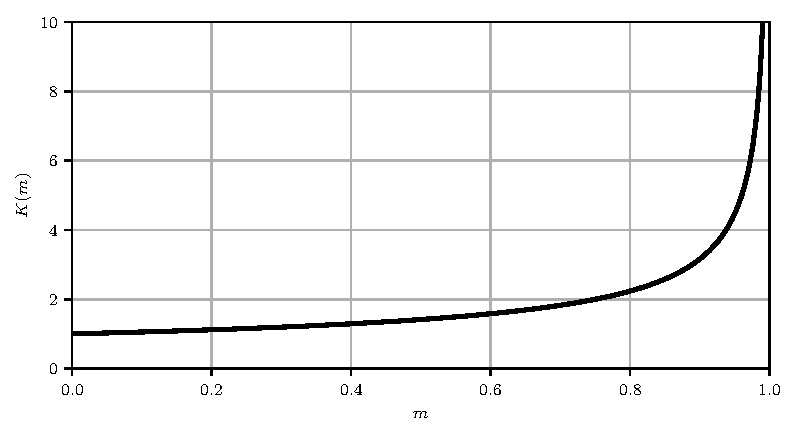
\includegraphics[scale=1]{meca/fonction_K.pdf}
    \vspace{-2em}
    \caption{Graphe de la fonction $K(m)$.}
\end{figure}
\end{exercise}

\begin{solution}
\begin{questions}
    \questioncours \'Equation du pendule $\Ddot{\theta} - k/m\sin\theta = 0$ d'où $\omega_0 = \sqrt{\dfrac{k}{m}}$.
    \question\begin{parts}
        \part Non linéarité et frottements.
        \part Idéal : cercles concentriques, réel sans frottement : des ovales rigolos, réel avec frottement : des spirales cheloues.
    \end{parts}
    \question\begin{parts}
        \part TMC depuis l'équation du pendule
        $$\dfrac{1}{2}\dv{}{t}\qty(\dot{\theta}^2) - {\omega_0}^2\sin\theta\dv{\theta}{t} = 0$$
        et par intégrale première du mouvement entre $\theta = \theta_0$ et $\theta(t)$ :
        $$\dot{\theta} = \omega_0\sqrt{\cos\theta_0 - \cos\theta}.$$
        \part D'où par intégration entre $0$ et $T/4$ et $0$ et $\theta_0$ :
        $$T = \dfrac{2T_0}{\pi}\int_{0}^{\theta_0}\dfrac{\dd{t}}{\sqrt{\cos\theta_0 - \cos\theta}}.$$
        et avec le changement de variable $\sin\phi = \dfrac{\sin(\theta/2)}{\sin(\theta_0/2)}$, on trouve $T = T_0 K(\sin^2(\theta_0)/2).$
        \part Pour $m$ petit,
        $$\frac{1}{\sqrt{1-m\sin^{2}\phi}}=1+\frac{\sin^{2}\phi}{2}m+\mathcal{O}(m^2\sin^{4}\phi),$$
        d'où par intégration on retrouve la formule de Borda.
        \part Le terme suivant, et on fait un critère.
    \end{parts}
\end{questions}
\end{solution}